\begin{abwframe}
\node[anchor=north west,inner sep=0pt,outer sep=0pt] at (40.625,-55.791) {\begin{minipage}[t][69.584bp][c]{878.75bp}\setlength{\parindent}{0pt}\setlength{\parskip}{0pt}{\TimesNR\fontsize{44}{49.28}\selectfont\color{cBC0031}\bfseries\raggedright Example: The AND Perceptron\par}\end{minipage}};
\node[anchor=north west,inner sep=0pt,outer sep=0pt] at (40.625,-158.857) {\begin{minipage}[t][294.114bp][c]{348.035bp}\setlength{\parindent}{0pt}\setlength{\parskip}{0pt}{\TimesNR\fontsize{24}{26.88}\selectfont\color{c000000}\raggedright Suppose we use the step function for activation.\par}{\TimesNR\fontsize{24}{26.88}\selectfont\color{c000000}\vphantom{Ag}\par}{\TimesNR\fontsize{24}{26.88}\selectfont\color{c000000}\raggedright Suppose Boolean value false is represented as number 0.\par}{\TimesNR\fontsize{24}{26.88}\selectfont\color{c000000}\vphantom{Ag}\par}{\TimesNR\fontsize{24}{26.88}\selectfont\color{c000000}\raggedright Suppose Boolean value true is represented as number 1.\par}{\TimesNR\fontsize{24}{26.88}\selectfont\color{c000000}\vphantom{Ag}\par}{\TimesNR\fontsize{24}{26.88}\selectfont\color{c000000}\raggedright Then, the perceptron on the right computes the Boolean AND function!\par}\end{minipage}};
\draw[fill=cD2CFD5,fill opacity=1,draw=c141215,line width=1bp,rotate around={0:(707.281,-278.592)}] (707.281,-278.592) ellipse [x radius=112.79bp,y radius=61.5bp];
\node[anchor=north west,inner sep=0pt,outer sep=0pt] at (601.691,-220.692) {\begin{minipage}[t][115.8bp][c]{211.18bp}\setlength{\parindent}{0pt}\setlength{\parskip}{0pt}{\TimesNR\fontsize{28}{31.36}\selectfont\color{c000000}\itshape\centering \ensuremath{z}=\ensuremath{h}  \ensuremath{\mathbf{w}} \ensuremath{T} \ensuremath{\mathbf{x}} \par}\end{minipage}};
\draw[fill=none,draw=cFF0000,line width=3bp,-{Stealth}] (427.545,-153.325) -- (627.526,-235.105);
\draw[fill=none,draw=c1F1D21,line width=3bp,-{Stealth}] (425.721,-289.894) -- (595.931,-319.527);
\draw[fill=none,draw=c1F1D21,line width=3bp,-{Stealth}] (424.838,-234.726) -- (597.442,-264.616);
\node[anchor=north west,inner sep=0pt,outer sep=0pt] at (383.176,-217.726) {\begin{minipage}[t][33.998bp][t]{34.463bp}\setlength{\parindent}{0pt}\setlength{\parskip}{0pt}{\TimesNR\fontsize{28}{31.36}\selectfont\color{c000000}\itshape\raggedright  \ensuremath{x} 1 \par}\end{minipage}};
\node[anchor=north west,inner sep=0pt,outer sep=0pt] at (384.082,-115.726) {\begin{minipage}[t][33.998bp][t]{86.925bp}\setlength{\parindent}{0pt}\setlength{\parskip}{0pt}{\TimesNR\fontsize{28}{31.36}\selectfont\color{c000000}\itshape\raggedright  \ensuremath{x} 0 =1\par}\end{minipage}};
\node[anchor=north west,inner sep=0pt,outer sep=0pt] at (383.407,-302.528) {\begin{minipage}[t][33.998bp][t]{35.114bp}\setlength{\parindent}{0pt}\setlength{\parskip}{0pt}{\TimesNR\fontsize{28}{31.36}\selectfont\color{c000000}\itshape\raggedright  \ensuremath{x} 2 \par}\end{minipage}};
\node[anchor=north west,inner sep=0pt,outer sep=0pt,rotate=-21.765] at (485.51,-160.278) {\begin{minipage}[t][33.998bp][t]{113.78bp}\setlength{\parindent}{0pt}\setlength{\parskip}{0pt}{\TimesNR\fontsize{28}{31.36}\selectfont\color{c000000}\itshape\raggedright  \ensuremath{w} 0 =\ensuremath{-}3\par}\end{minipage}};
\node[anchor=north west,inner sep=0pt,outer sep=0pt,rotate=-9.98] at (445.096,-208.584) {\begin{minipage}[t][33.998bp][t]{92.05bp}\setlength{\parindent}{0pt}\setlength{\parskip}{0pt}{\TimesNR\fontsize{28}{31.36}\selectfont\color{c000000}\itshape\raggedright  \ensuremath{w} 1 =2\par}\end{minipage}};
\node[anchor=north west,inner sep=0pt,outer sep=0pt,rotate=-350.399] at (439.016,-271.553) {\begin{minipage}[t][33.998bp][t]{92.701bp}\setlength{\parindent}{0pt}\setlength{\parskip}{0pt}{\TimesNR\fontsize{28}{31.36}\selectfont\color{c000000}\itshape\raggedright  \ensuremath{w} 2 =2\par}\end{minipage}};
\draw[fill=none,draw=c1F1D21,line width=3bp,-{Stealth}] (820.071,-278.592) -- (928.746,-278.592);
\node[anchor=north west,inner sep=0pt,outer sep=0pt] at (821.678,-239.494) {\begin{minipage}[t][33.998bp][t]{110.564bp}\setlength{\parindent}{0pt}\setlength{\parskip}{0pt}{\TimesNR\fontsize{28}{31.36}\selectfont\color{c000000}\raggedright Output: \ensuremath{z}\par}\end{minipage}};
\node[anchor=north west,minimum width=243.106bp,minimum height=123.595bp,inner sep=0pt,fill=none,draw=c000000,line width=0.75bp] at (648.996,-44.74) {};
\node[anchor=north west,inner sep=0pt,outer sep=0pt] at (656.196,-48.34) {\begin{minipage}[t][116.395bp][t]{228.706bp}\setlength{\parindent}{0pt}\setlength{\parskip}{0pt}{\TimesNR\fontsize{24}{26.88}\selectfont\color{c000000}\bfseries\raggedright false AND false = false\par}{\TimesNR\fontsize{24}{26.88}\selectfont\color{c000000}\bfseries\raggedright false AND true = false\par}{\TimesNR\fontsize{24}{26.88}\selectfont\color{c000000}\bfseries\raggedright true AND false = false\par}{\TimesNR\fontsize{24}{26.88}\selectfont\color{c000000}\bfseries\raggedright true AND true = true\par}\end{minipage}};
\node[anchor=north west,inner sep=0pt,outer sep=0pt] at (56.693,-499.702) {\begin{minipage}[t][11.952bp][c]{324bp}\setlength{\parindent}{0pt}\setlength{\parskip}{0pt}{\TimesNR\fontsize{10}{11.2}\selectfont\color{c7F7F7F}\raggedright Analytics for a Better World Lecture 2\par}\end{minipage}};
\node[anchor=north west,inner sep=0pt,outer sep=0pt] at (880.898,-499.702) {\begin{minipage}[t][11.952bp][c]{22.409bp}\setlength{\parindent}{0pt}\setlength{\parskip}{0pt}{\TimesNR\fontsize{10}{11.2}\selectfont\color{c7F7F7F}\bfseries\raggedleft 22\par}\end{minipage}};
\node[anchor=north west,inner sep=0pt,outer sep=0pt] at (402.504,-346.758) {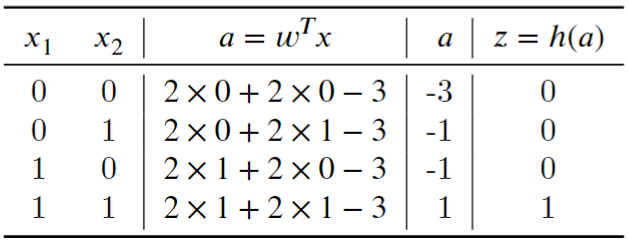
\includegraphics[width=471.816bp,height=180.775bp]{assets/source/slide-22-object-007.png}};
\end{abwframe}
